\documentclass[10pt]{article}
\usepackage[margin=2.2cm]{geometry}
\usepackage{amsmath}
\usepackage{graphicx}
\usepackage{enumitem}
\usepackage[hidelinks]{hyperref}
\setlength{\parindent}{0pt}
\setlength{\parskip}{5pt}

\title{\vspace{-1.2cm}Reading the onset-hazard vs.\ intensity overlay\\
\large Budget-pressure reward-hacking experiment (\texttt{hack\_intensity\_vs\_fraction\_used.pdf})}
\date{}

\begin{document}
\maketitle
\vspace{-1.4cm}

\textbf{Setup.} For each at-risk API turn at budget pressure $x$ (fraction of budget used), define
three per-turn rates:
\begin{align*}
h(x) &= \Pr(\text{\emph{first} hack at this turn} \mid \text{run still clean}) && \text{\emph{onset hazard} (red, dashed)}\\
r(x) &= \Pr(\text{\emph{another} hack at this turn} \mid \text{run already hacked}) && \text{\emph{post-onset rate} (green, dotted)}\\
\lambda(x) &= \Pr(\text{\emph{any} hack action at this turn}) && \text{\emph{intensity} (blue, solid)}
\end{align*}
With $w(x)$ the share of at-risk turns at pressure $x$ belonging to still-clean runs,
\[
\lambda(x) \;=\; w(x)\,h(x) \;+\; \bigl(1-w(x)\bigr)\,r(x),
\]
i.e.\ the observed intensity is a mixture of the two conditional rates, weighted by how much of
the population is still clean. The pipeline plots all three on
\texttt{hack\_intensity\_vs\_fraction\_used.pdf}; the underlying rows (with a
\texttt{post\_onset} flag) are in \texttt{person\_period\_recurrent.csv}.

\begin{center}
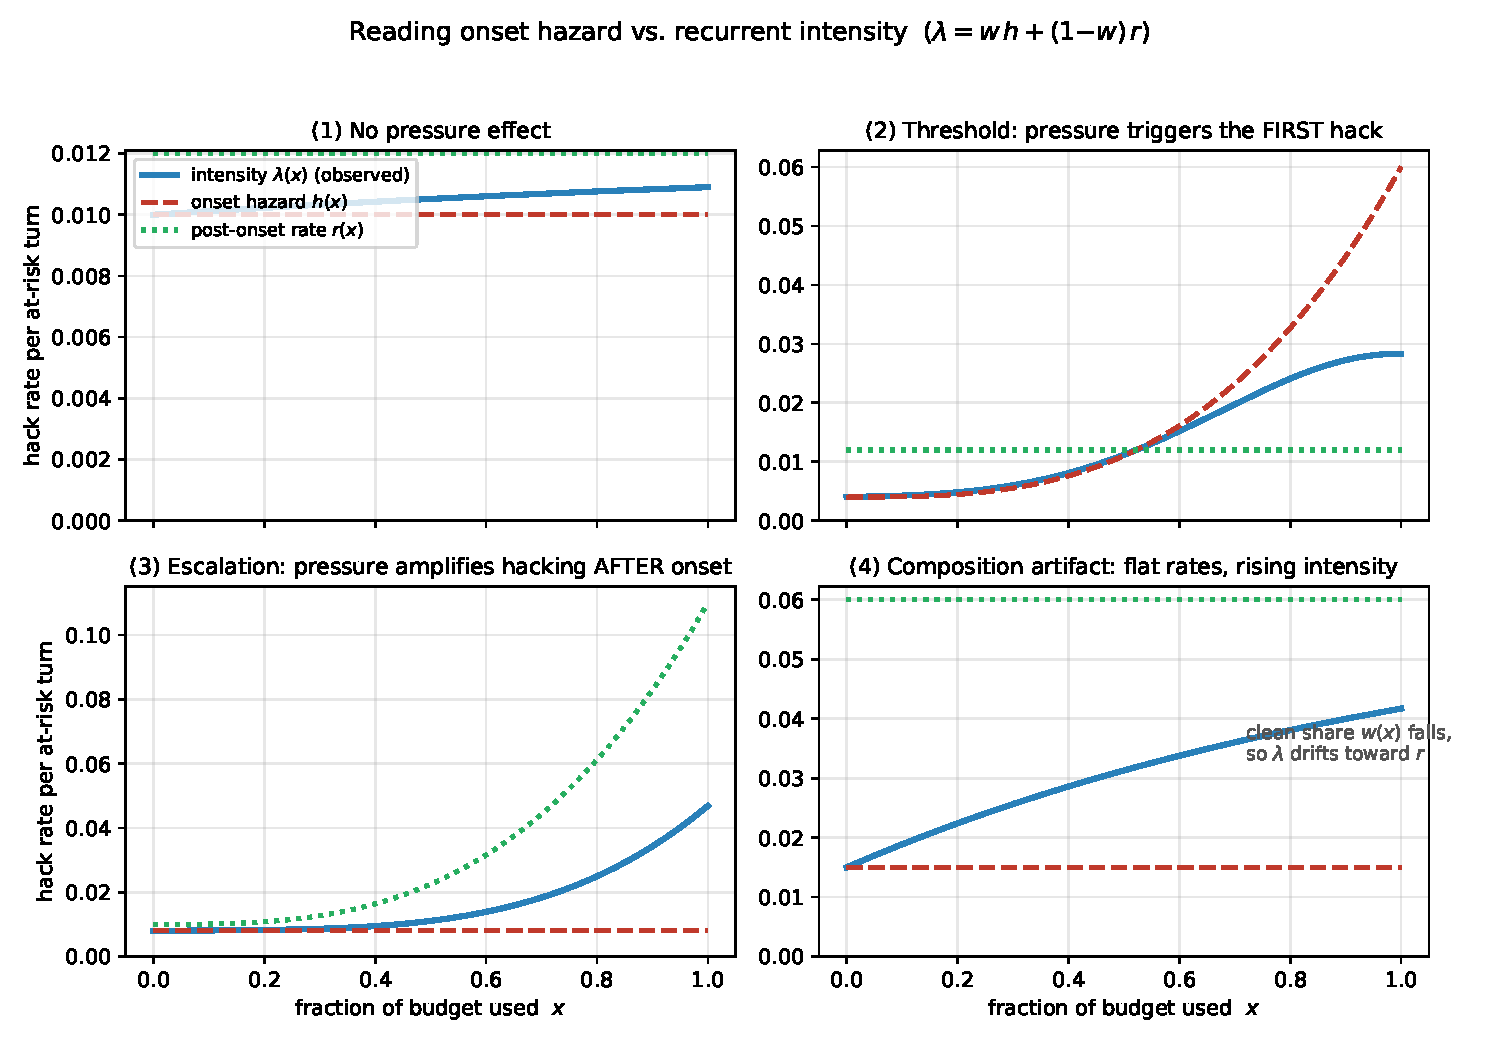
\includegraphics[width=\textwidth]{onset_vs_intensity_panels.pdf}
\end{center}

\begin{description}[leftmargin=1.6em, style=nextline]

\item[(1) No pressure effect.] All three rates are flat in $x$: hacking (if any) is a constant
per-turn propensity, driven by something other than the budget (e.g.\ task frustration).
Budget pressure is not a causal factor; the per-trajectory hacking rate still grows with budget,
but only because longer runs accumulate more flat-rate exposure.

\item[(2) Threshold mechanism.] The onset hazard $h$ rises toward exhaustion while the
post-onset rate $r$ stays flat: pressure makes a still-clean agent more likely to cross the line
for the \emph{first} time, and does nothing further once the line is crossed. Intensity rises
while clean runs dominate the population ($w\approx1$), but as onsets accumulate and $w$ falls,
$\lambda$ bends back toward the flat $r$ --- in a pure-threshold world, observed intensity can
\emph{understate} late-budget onset risk. \emph{Signature: the red curve itself rises.}
(If pressure instead raised \emph{everyone's} propensity uniformly --- $h$ and $r$ rising
together --- that is the conjunction of (2) and (3), and the green curve distinguishes the two.)
Intervention target: the late-budget decision point of clean agents (e.g.\ reframing the budget
reminder near exhaustion).

\item[(3) Escalation mechanism.] Onset $h$ stays flat --- pressure does \emph{not} make the first
transgression more likely --- but the post-onset rate $r$ rises steeply: once an agent has hacked,
pressure amplifies further hacking (the line-crossing cost is paid; the hack persists in the repo
and in the agent's context). The blue curve separates upward from the flat red curve.
\emph{Signature: $\lambda$ rises while $h$ is flat \underline{and} $r$ rises.} Intervention
target: the first violation, whenever it occurs --- monitoring should escalate sharply after it.

\item[(4) Composition artifact (the trap).] All \emph{conditional} rates are flat ($h$ low, $r$
elevated but constant: no escalation), yet the observed intensity $\lambda$ still climbs. Reason:
onsets accumulate as runs progress, so the clean share $w(x)$ falls with $x$ and the mixture
drifts from $h$ toward the higher $r$ --- a population-composition effect, not a behavioral
response to pressure. Panels (3) and (4) are \textbf{indistinguishable from the blue and red
curves alone}; only the green post-onset rate separates them ($r$ rising in (3), flat in (4)).
This is why a rising intensity must never be reported as ``pressure escalates hacking'' without
checking $r(x)$ directly.

\end{description}

\textbf{Reading rule.} Rising red $\Rightarrow$ threshold effect on first transgressions.
Rising blue with flat red $\Rightarrow$ compute $r(x)$ before concluding anything: rising green
confirms escalation; flat green means composition. Flat everything $\Rightarrow$ no
pressure effect. (A fifth case, red and green both rising, is the conjunction of (2) and (3).)
Caveat: even a genuinely rising $r$ admits a selection reading --- hack-prone runs accumulate in
the post-onset population --- so confirming \emph{state-dependence} (``crossing changed the
agent'') requires within-run before/after comparison, which the person-period tables support
given enough repeat events.

\end{document}
